\documentclass[spanish]{article}
\usepackage[spanish]{babel}
\usepackage[utf8]{inputenc}
\usepackage{mathtools}
\usepackage{graphicx,float}
\usepackage{amsfonts,txfonts}
\usepackage[colorlinks, urlcolor=blue]{hyperref}
\usepackage[top = 1.5cm, bottom = 1.5cm, left = 2cm, right = 2cm]{geometry}


\title{Presentación de Avance - Proyecto SWE \\ILI384: Taller de Modelos y Métodos Cuantitativos}
\author{Rodrigo Naranjo \and Martín Villanueva}
\date{5 de Enero 2016}

\begin{document}
\maketitle

\thispagestyle{empty}


\section{Descripción del Problema}
El problema consiste en modelar el sistema de \textit{Shallow Water Equations} en $1D$ y $2D$, de tal modo
que se pueda determinar la evolución del sistema, dadas las ecuaciones diferenciales que modelan el problema,
las condiciones iniciales y las condiciones de borde. Las SWE corresponden a un caso particular de las ecuaciones
de Navier-Stokes, que se obtienen al hacer la suposición de que el fluido es incompresible y que no existe viscosidad, aunque esta última puede relajarse para obtener un sistema más realista. En el caso general (2D) las ecuaciones pueden
escribirse como a continuación
\begin{align}
\begin{split}
 & \frac{\partial u}{\partial t} + u \frac{\partial u}{\partial x} + v \frac{\partial u}{\partial y} + g \frac{\partial h}{\partial x} = 0 \\
 & \frac{\partial v}{\partial t} + u \frac{\partial v}{\partial x} + v \frac{\partial v}{\partial y} + g \frac{\partial h}{\partial y} = 0 \\
 & \frac{\partial h}{\partial t} + \frac{\partial }{\partial x}(u(h-b)) + \frac{\partial }{\partial y}(v(h-b)) = 0
\end{split}
\end{align}
donde las variables de interés (a modelar) son $h(x,y,t)$ (nivel de agua), $u(x,y,t)$ (componente de velocidad de una columna de
agua en $x$), $v(x,y,t)$ (componente de velocidad de una columna de agua en $y$). Adicionalmente deben ser conocidos $b(x,y)$, que corresponde a la \textit{batimetría} que describe la forma del fondo marino  y las condiciones de borde e iniciales del sistema.

\begin{figure}[htpb!]
\centering
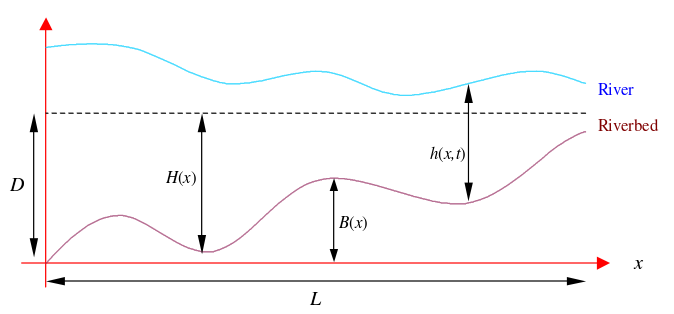
\includegraphics[scale=0.6]{schematic.png}
\caption{Esquema de SWE en una dimensión.}
\end{figure}

\section{La Implementación}
Para la resolución del problema se plantea un enfoque del tipo partículas, similar a \textit{Shallow Water Particles} \cite{swp} donde la superficie del agua se modela por medio de la distribución que tome este conjunto de partículas. En el enfoque aquí propuesto, cada una de las variables de interés ($h$, $u$ y $v$) se aproximan como una combinación lineal de funciones RBF
\begin{align}
 \sum_{i=1}^{N} \gamma_i(t)\Phi(||\mathbf{x}-\boldsymbol{\xi}_i(t)||, \epsilon_i(t))    
\end{align}
 
\noindent donde la función RBF a ocupar es de preferencia una función de soporte compacto, de modo que se acote el radio de influencia de cada partícula, y se generen de este modo sistemas \textit{sparse}.

Lo que se quiere lograr sigue el enfoque \textit{Evolutive RBF} como en \cite{rossi}, donde se obtienen ecuaciones de evolución (ODE system) para los parámetros dependientes del tiempo en cada RBF ($\gamma(t)$, $\boldsymbol{\xi}_i(t)$ y $\epsilon_i(t)$). Las ventajas de esto, es que para obtener el estado del sistema en un tiempo $t+\Delta t$, requiere tan sólo computar las ecuaciones de evolución para cada RBF (de cada variable) y luego sumar los resultados respectivos en el espacio.

La implementación de la solución espera ser incremental, abordando la complejidad del problema paso por paso. En base a esto, se planea seguir el siguiente orden.

\begin{enumerate}
\item Inicialmente se propone resolver las \emph{Burgers' Equations} en 1D sin viscosidad, definidas por:
\begin{align}
\frac{\partial u}{\partial t} + u\frac{\partial u}{\partial x} = 0
\label{eq:burger}
\end{align}
que es de interés pues es no lineal y se deriva de un modelo de convección-difusión, por lo tanto muy similar a las SWE.

\item El siguiente paso, consiste en resolver las SWE en 1D, a modo de obtener una idea de las propiedades y comportamiento de la solución propuesta, antes de avanzar a más dimensiones. Para este paso se pretende ocupar en primer lugar funciones RBF gaussianas, para luego dar con alguna implementación con funciones de soporte compacto.

\item Implementar la solución anterior al problema en 2D, considerando movimiento en el eje X e Y.

\item Implementar condiciones de borde, iniciales y batimetría utilizadas (por otros métodos de simulación) y probarlos con esta solución para establecer comparaciones, y verificar si se están obteniendo resultados correctos.

\item Posiblemente también será necesario agregar los términos de viscosidad al sistema, para analizar sus efectos y obtener resultados más realistas.

\item Buscar métodos para optimizar la ejecución de la solución encontrada: Paralelización/Implementación en GPU, Fast multipole method, aprovechar propiedades del sistema sparse, entre otras.
\end{enumerate}


\section{Dificultades}
Se presentan aquí algunas de las dificultades que se conocen, y otras que eventualmente podrían aparecer en la implementación
del proyecto.
\begin{itemize}
    \item La batimetría $b(x,y)$ es, en general, una función discontinua (o que se conoce parcialmente), y por lo tanto
    debe hallarse una manera de aproximar sus derivadas.
    \item En simulaciones ocupando otros métodos (SPH \textit{Smoothed Particle Hydrodynamics}), se ha notado que no tomar
    en cuenta la viscosidad, puede llevar a problemas de estabilidad numérica en las simulaciones.
    \item Probablemente en las simulaciones sea necesario ocupar una gran cantidad de partículas para modelar la superficie
    del agua, lo cual lleva a una gran cantidad de computación para determinar los estados siguientes del sistema. Por ello,
    quizás sea necesario paralelizar la ejecución, o buscar métodos más eficientes de computación (FMM Fast Multipole
    Method).
\end{itemize}                                                                                                                                                                                                                                                                                                                                                                                                     
\newpage  
\section{Burgers' Equation}
  \subsection{Análisis Teórico}
    Para realizar una prueba preliminar antes de modelar las SWE, se procedió a resolver la Burgers' Equation (\ref{eq:burger}), una ecuación que explica de manera simplificada el comportamiento de un fluido incompresible, por medio de las leyes de la conservación. Para realizar esto se define una solución $u(x,t)$ como una combinación lineal de RBFs, del siguiente modo
    \begin{align}
      u(x,t) = \sum_{i} \phi_{h_i}(x,t) = \sum_i \gamma_i(t)\phi_{h_i}(x-\xi_i(t),\epsilon_i)
    \end{align}
    
    \noindent donde se utiliza $\displaystyle \phi(x,\epsilon) = e^{-(\epsilon x)^2}$. Siguiendo el enfoque \textit{evolutivo} se propone a cada $\Phi(x,t)$ (se omite subíndice por simplicidad) como solución de (\ref{eq:burger}), sin embargo para abordar el problema de la no linealidad, debe hacer una modificación al problema inicial. En vista de que se propone a $\Phi(x,t)$ como una solución a la PDE, es razonable aproximar $u(x,t)$ como una expansión de Taylor en torno a $(\xi(t),t)$ obteniendo
    \begin{align}
      u(x,t) = u(\xi(t),t) + \frac{u_x(\xi(t),t)}{1!}(x-\xi(t)) + \cdots
    \end{align}
    si tomamos sólo el primer término de esta expansión (de orden cero), y  se reemplaza la solución propuesta $\Phi(x,t)$, entonces se obtiene
    \begin{align}
      \frac{\partial}{\partial t}\Phi(x-\xi(t),\epsilon(t)) + u(\xi(t),t)\ \frac{\partial}{\partial x}\Phi(x-\xi(t),\epsilon(t)) = 0
      \label{eq:burgersimple}
    \end{align}

    \noindent luego realizando el álgebra necesaria en (\ref{eq:burgersimple}), se obtienen las siguientes ecuaciones de evolución para los parámetros de cada RBF
    \begin{align*}
    & \epsilon'(t) = 0 \\
    & \gamma'(t) = 0  \\
    & \xi'(t) = u(\xi(t),t)
    \end{align*}
   
    \noindent este sistema dice que cada una de las partículas mantiene su su forma y peso, pero que sin embargo pueden cambiar su posición (centro) en el tiempo, y por lo tanto la altura de la columna de agua en cada punto estará determinada sólo por la distribución de las partículas.


    \subsection{Análisis experimental}
    Se realizó un experimento modelando el comportamiento de la ecuación para el estado inicial $u(x,0) = I_{x \in [8,12]}\frac{(8-x)(x-12)}{12}$ como se muestra a continuación

    \begin{figure}[H]
        \centering
        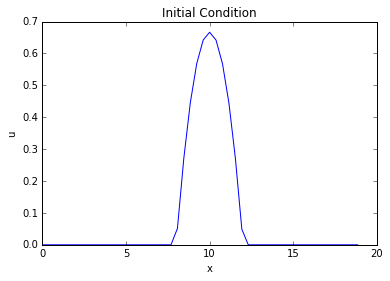
\includegraphics[scale=0.6]{initialu.png}
    \end{figure}
    

    Computando simultáneamente las ecuaciones de evolución para cada una de las RBF, y luego sumando la combinación lineal en cada time step, se obtiene entonces la aproximación de la solución en el tiempo. Como se vio anteriormente el único parámetro que realmente varía es $\xi(t)$, que es la posición del centro de cada partícula. A continuación se muestra la evolución de cada uno de estos centros para un sistema de $20$ partículas
    \begin{figure}[H]
      \centering
      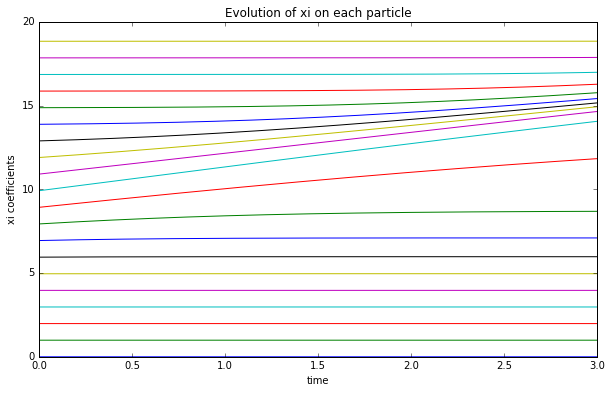
\includegraphics[scale=0.5]{xis.png}
    \end{figure}
    
    Algunos resultados obtenidos para la evolución de la ecuación en el tiempo son los que se muestran a continuación: \\
    \begin{figure}[H]
      \centering
      \begin{minipage}{.5\textwidth}
        \centering
        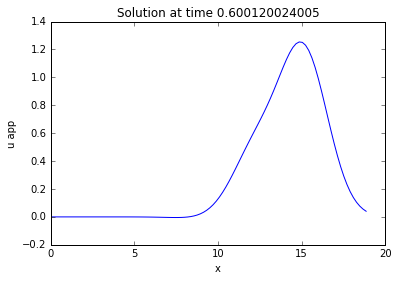
\includegraphics[scale=0.6]{t1000.png}
      \end{minipage}%
      \begin{minipage}{.5\textwidth}
        \centering
        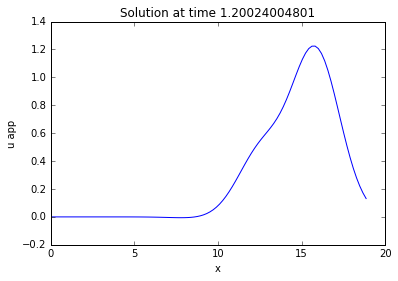
\includegraphics[scale=0.6]{t2000.png}
      \end{minipage}
    \end{figure}
    \begin{figure}[H]
      \centering
      \begin{minipage}{.5\textwidth}
        \centering
        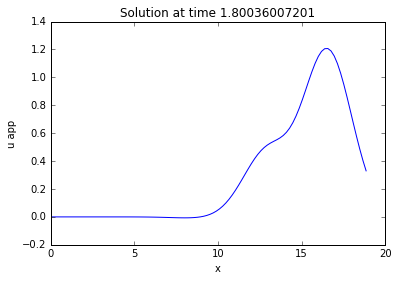
\includegraphics[scale=0.6]{t3000.png}
      \end{minipage}%
      \begin{minipage}{.5\textwidth}
        \centering
        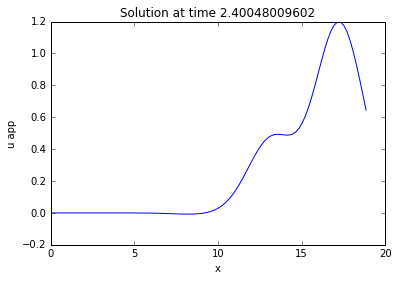
\includegraphics[scale=0.6]{t4000.png}
      \end{minipage}
    \end{figure}
    \begin{figure}[H]
      \centering
      \begin{minipage}{.5\textwidth}
        \centering
        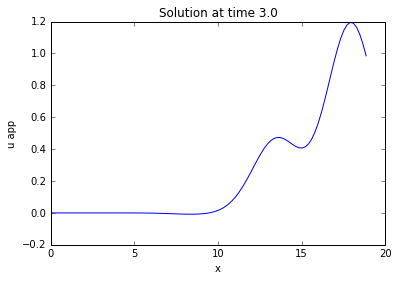
\includegraphics[scale=0.6]{t5000.png}
      \end{minipage}%
    \end{figure}
    Tal como se observa, el comportamiento modelado por la \textit{Burgers' Equation} es bastante simple, consistiendo en un
    movimiento de la perturbación inicial $u(x,0)$ hacia la derecha. Algunos de los detalles que pudieron
    observarse en la simulación, son la aparición de una perturbación más pequeña que parece moverse a menor velocidad que el
    resto del sistema. Tales problemas pueden ser abordados por medio de \textit{remeshing}, esto es, pasado un intervalo de tiempo volver a realizar una interpolación RBF, para estabilizar las posiciones y velocidades del sistema.
    
    \section{Evolutive Shallow Water Equations}

    \subsection{Derivación en 1D}

    El sistema a resolver corresponde a la versión 1D de las SWE, tomando por simplicidad la restricción de que la batimetría es constante y cero $b(x)=0$, respecto al nivel de referencia. Así el sistema a trabaja es
\begin{align}
 & \frac{\partial h}{\partial t} + h \frac{\partial u}{\partial x} + u \frac{\partial h}{\partial x} = 0 \label{eq:continuity}\\
 & \frac{\partial u}{\partial t} + u \frac{\partial u}{\partial x} + g \frac{\partial h}{\partial x} = 0 \label{eq:momentum}
\end{align}

    Tal como se hizo anteriormente para la \textit{Burgers' Equation}, se proponen como solución al sistema anterior, las siguientes dos funciones respectivamente:

\begin{align}
     & h(x,t) = \sum_{i=1}^{N} \gamma_h(t)\phi(x-\xi_h(t),\epsilon_h(t)) + H_0 \label{eq:happ}\\
     & u(x,t) = \sum_{i=1}^{N} \gamma_u(t)\phi(x-\xi_u(t),\epsilon_u(t)) + U_0 \label{eq:uapp}
 \end{align}

     donde $H_0$ y $U_0$ son constantes, que denotaremos \textit{Sea level} y \textit{Base velocity}. La idea es que la
     combinación lineal de RBFs en cada caso, capturen las variaciones por sobre los niveles base establecidos, dando así
     más estabilidad al enfoque evolutivo.

     Para la derivación, consideraremos en primer lugar reemplazar la solución propuesta (\ref{eq:happ}) en (\ref{eq:continuity}), tomando como conocidos $u$ y $u_x$ en un tiempo dado
     \begin{align*}
     \sum_{i=1}^{N} \frac{\partial}{\partial t}[\gamma_{h_i}\phi_{h_i}(x)] + \left(\sum_{i=1}^{N} \gamma_{h_i} \phi_{h_i}(x) + H_0\right) u_x + u \sum_{i=1}^N \frac{\partial}{\partial x}[\gamma_{h_i}\phi_{h_i}(x)] & = 0 \\
     \sum_{i=1}^{N} \frac{\partial}{\partial t}[\gamma_{h_i}\phi_{h_i}(x)] + \sum_{i=1}^{N} \gamma_{h_i} \phi_{h_i}(x)u_x + H_0 u_x +  \sum_{i=1}^N u \frac{\partial}{\partial x}[\gamma_{h_i}\phi_{h_i}(x)] & = 0 \\
     \sum_{i=1}^{N} \frac{\partial}{\partial t}[\gamma_{h_i}\phi_{h_i}(x)] + \sum_{i=1}^{N} \gamma_{h_i} \phi_{h_i}(x)u_x + \sum_{i=1}^{N} \frac{H_0 u_x}{N} +  \sum_{i=1}^N u \frac{\partial}{\partial x}[\gamma_{h_i}\phi_{h_i}(x)] & = 0 \\
     \sum_{i=1}^N \left(\frac{\partial}{\partial t}[\gamma_{h_i}\phi_{h_i}(x)] + \left(\gamma_{h_i} \phi_{h_i}(x) + \frac{H_0}{N}\right)u_x + u \frac{\partial}{\partial x}[\gamma_{h_i}\phi_{h_i}(x)]\right) & = 0
     \end{align*}

     \noindent aquí se simplifica la notación $\displaystyle \gamma_{h_i}\phi_{h_i}(x) = \gamma_{h_i}(t)\phi(x-\xi_{h_i}(t),\epsilon_{h_i}(t))$. Adicionalmente se agrega una sumatoria sobre $H_0$ para poder formar una sola suma. De la última ecuación obtenida, se desprende que si cada partícula o RBF cumple con
     \begin{align}
          \frac{\partial}{\partial t}[\gamma_{h_i}\phi_{h_i}(x)] + \left(\gamma_{h_i} \phi_{h_i}(x) + \frac{H_0}{N}\right)u_x + u \frac{\partial}{\partial x}[\gamma_{h_i}\phi_{h_i}(x)] = 0
          \label{eq:simplcont}
      \end{align}

      \noindent entonces su combinación lineal será una solución de (\ref{eq:continuity}). En (\ref{eq:simplcont}) se aproximan $u$ y $u_x$ por los valores en los centros de las RBFs, esto es, $u \approx u(\xi(t),t)$ y $u_x \approx u_x(\xi(t),t)$ (Aproximación de Taylor de orden $0$). Tal como lo interpreta L. Rossi en \cite{rossi}, esto quiere decir que para cada partícula, estamos aproximando su velocidad por la velocidad en su centro. Por lo tanto, mientras más amplio sea el alcance de cada partícula, mayor será el error que se está cometiendo en la aproximación de la velocidad.

      Una derivación equivalente puede realizarse para $u(x,t)$, el reemplazar (\ref{eq:uapp}) en (\ref{eq:momentum}), esta vez tomando como conocidos $u$ y $h_x$ en un tiempo dado
      \begin{align*}
      \sum_{i=1}^{N} \frac{\partial}{\partial t}[\gamma_{u_i}\phi_{u_i}(x)] + u  \left(\sum_{i=1}^{N}\frac{\partial}{\partial x} [\gamma_{u_i} \phi_{u_i}(x)]\right) + g \ h_x & = 0 \\
      \sum_{i=1}^{N} \frac{\partial}{\partial t}[\gamma_{u_i}\phi_{u_i}(x)] + \left(\sum_{i=1}^{N}u \frac{\partial}{\partial x} [\gamma_{u_i} \phi_{u_i}(x)]\right) + \sum_{i=1}^N \frac{g \ h_x}{N} & = 0 \\
      \sum_{i=1}^{N}\left( \frac{\partial}{\partial t}[\gamma_{u_i}\phi_{u_i}(x)] + u \frac{\partial}{\partial x} [\gamma_{u_i} \phi_{u_i}(x)] + \frac{g \ h_x}{N} \right) & = 0
      \end{align*}

      \noindent donde se realiza la misma simplificación de notación, y el mismo truco para sumar $g h_x$. Del mismo modo que antes, si cada partícula cumple con  
      \begin{align}
          \frac{\partial}{\partial t}[\gamma_{u_i}\phi_{u_i}(x)] + u \frac{\partial}{\partial x} [\gamma_{u_i} \phi_{u_i}(x)] + \frac{g \ h_x}{N} = 0
          \label{eq:simplmom}
      \end{align}

      \noindent entonces su combinación lineal será una solución de  (\ref{eq:momentum}). En (\ref{eq:simplmom}) se aproximan $u$ y $h_x$ por los valores en los centros de las RBFs, generando el mismo tipo de error que antes.


      Reemplazando las RBFs respectivas (Gaussianas) en (\ref{eq:simplcont}) y (\ref{eq:simplmom}), desarrollando el álgebra necesaria, y realizando las siguientes dos aproximaciones
      \begin{align*}
          e^{\epsilon_h(t)^2 (x-\xi_h(t))^2} & = 1 + \epsilon_h(t)^2 (x-\xi_h(t))^2 + O([x-\xi_h(t)]^3) \\
          e^{\epsilon_u(t)^2 (x-\xi_u(t))^2} & = 1 + \epsilon_u(t)^2 (x-\xi_u(t))^2 + O([x-\xi_u(t)]^3)
      \end{align*}
      por series de Taylor centradas en $\xi_h(t)$ y $\xi_u(t)$ respectivamente, se obtiene el sistema dinámico (\ref{eq:system}) con las ecuaciones que definen la evolución de los parámetros, para las partículas de $h$ y $u$
     \begin{align}
     \begin{split}
    \gamma _h'(t) &= -\left(\frac{H}{N} + \gamma _h(t)\right)u_x  \\
    \xi _h'(t) &= u \\
    \epsilon _h'(t) &= \frac{H \ u_x \ \epsilon_h(t)}{2 N \ \gamma_h(t)} \\
    \gamma _u'(t) &= -\frac{g h_x}{N} \\
    \xi _u'(t) &= u \\
    \epsilon _u'(t) &= \frac{g \ h_x \ \epsilon _u(t)}{2 N \ \gamma_u(t)}
    \end{split}
    \label{eq:system}
    \end{align}

    Existen varios detalles interesantes en este sistema, y que se comentan a continuación:

    \begin{enumerate}
        \item Aunque pareciera que el sistema (\ref{eq:system}) está desacoplado (los parámetros de $h$ no dependen de los de $u$, y viceversa) esto no es así, pues los parámetros $\gamma_h, \xi_h, \epsilon_h$ dependen de $u$ y $u_x$, y los parámetros $\gamma_u, \xi_u, \epsilon_u$ dependen de $h_x$.
        \item Las velocidades de las partículas/RBF's de $h$ y $u$ se mueven con la misma velocidad en su centro ($\xi_h'(t) = \xi_u'(t) = u$). Tomando en cuenta que además se ocupan la misma cantidad de partículas en cada caso ($N$), y con los mismos centros iniciales (detalle de implementación), esto implica que en todo tiempo exista una correspondencia una a uno, entre partículas de $h$ y partículas de $u$.
        \item A diferencia de las ecuaciones de evolución obtenidas para la \textit{Burgers' Equation}, aquí los parámetros $\gamma$ y $\xi$ respectivos sí evolucionan. Esto difiere también del concepto de partícula planteado en \textit{SWP} \cite{swp}, donde las partículas de $h$ no pueden cambiar su peso ni su forma, cumpliendo por definición la ecuación de continuidad.
        \item Es importante notar que en la ecuación de evolución para $\epsilon$, en ambos casos aparece en el denominador $\gamma_h$ y $\gamma_u$ respectivamente. Por lo tanto, estas dos ecuaciones deben tratarse con especial cuidado para no caer en indeterminaciones. Una posible forma de abordar este problema, es estableciendo los niveles base $H_0$ y $U_0$ por debajo del valor mínimo en cada caso.
        \item Es interesante notar cómo se autorregulan los parámetros $\gamma_h$ y $\epsilon_h$ para satisfacer la condición de continuidad. Si $\gamma_h \rightarrow 0$ entonces $\epsilon_h \rightarrow \infty$, lo cual quiere decir que si una partícula disminuye su peso/altura, entonces se distribuye en una extensión espacial más amplia (distribuye su masa de acuerdo a su altura).  
    \end{enumerate}

    \subsection{Simulación en 1D}

    El proceso de simulación se compone básicamente de la ejecución de tres pasos: \textbf{Evolución}, \textbf{Reconstrucción} y \textbf{Verificación}.

    \begin{enumerate}
        \item \textbf{Evolución.} \  En cada time step, será necesario hacer evolucionar los parámetros de todas las partículas/RBFs del sistema, hacia los valores en un tiempo siguiente. Debido a que estas están desacopladas, esta operación es fácilmente vectorizable o paralelizable. Por lo demás son operaciones de muy bajo costo computacional, siendo esta la gran ventaja del enfoque evolutivo.
        \item \textbf{Reconstrucción.} \ Con los valores de cada uno de los parámetros en un tiempo siguiente, ahora es posible reconstruir las funciones $u$, $u_x$, $h$ y $h_x$ como la combinación lineal de las correspondientes partículas. Esto es necesario, pues se debe conocer los valores de estas funciones en las posiciones de los centros de las partículas.
        \item \textbf{Verificación.} \ Este paso corresponde a verificar la calidad de la soluciones obtenida en cada tiempo, estableciendo las condiciones bajo las cuales es necesario hacer \textit{remeshing}. Algunas condiciones posibles son:

        \begin{enumerate}
            \item Si $\gamma=0$ para alguna partícula de $h$ o $u$, entonces el sistema (\ref{eq:system}) se indetermina. Para resolver este problema se puede intentar bajar el nivel base $H_0$ o $U_0$, como alternativa al \textit{remeshing}.
            \item Como se analizó en la sección de derivación, la precisión espacial de nuestra solución está limitada por la extensión de cada una de las RBFs, vale decir, el método posee un error espacial $\displaystyle O(1 / \epsilon_{\text{min}}^2)$ \footnotemark[1]. Por lo tanto si en alguna de las partículas (tanto para $h$ como $u$), ocurre que $\epsilon \rightarrow 0$, nos indica que nuestra solución va por mal camino.
            \item El otro problema ocurre cuando las partículas empiezan a separarse considerablemente entre sí, formando \textit{gaps} (algo como lo que sucedió en las simulaciones de \textit{Burgers' Equation}). Para esto se puede establecer una distancia máxima entre partículas adyacentes $|\xi_i(t)-\xi_{i+1}(t)| \leq D_{\text{max}}$, la cual una vez sobrepasada hace necesario hacer \textit{remeshing}.
        \end{enumerate}
    \end{enumerate}

    El proceso de \textit{remeshing}, consiste en volver a la solución en el tiempo anterior, y realizar una interpolación $RBF$ en esta tal como si fuese una condición inicial. Luego se sigue evolucionando a partir de los valores de los parámetros que se obtengan en esta interpolación.

\footnotetext[1]{El orden del término $1/\epsilon_{\text{min}}$ se supone cuadrático, debido a que el procedimiento seguido es análogo al de L. Rossi \cite{rossi}, sin embargo esto debe ser demostrado.}


\newpage
\bibliography{ent3}
\bibliographystyle{ieeetr} 

\vfill\hfill RN/MV/\LaTeXe
\end{document}